\documentclass[sigconf, nonacm]{acmart}

\usepackage{amsmath,amsfonts}
\usepackage{graphicx}
\usepackage{textcomp}
\usepackage{multirow}
\usepackage{xcolor,colortbl}
\usepackage{algorithmic, algorithm}
\usepackage{caption}
\usepackage{subcaption}
\usepackage{xspace}
\usepackage{hyperref} % makes cross-refs (biblio, figures, algos, ...) clickable

%% The following content must be adapted for the final version
% paper-specific
\newcommand\vldbdoi{XX.XX/XXX.XX}
\newcommand\vldbpages{XXX-XXX}
% issue-specific
\newcommand\vldbvolume{14}
\newcommand\vldbissue{1}
\newcommand\vldbyear{2020}
% should be fine as it is
\newcommand\vldbauthors{\authors}
\newcommand\vldbtitle{\shorttitle}
% leave empty if no availability url should be set
\newcommand\vldbavailabilityurl{http://vldb.org/pvldb/format_vol14.html}
% whether page numbers should be shown or not, use 'plain' for review versions, 'empty' for camera ready
\newcommand\vldbpagestyle{plain}

\newcommand{\logic}[1]{\color{red}\textbf{Logic/flow:}#1\color{black}}
\newcommand{\writing}[1]{\color{green}\textbf{Writing:}#1\color{black}}
\newcommand{\tristan}[1]{\color{orange}\textbf{From Tristan:}#1\color{black}}
\newcommand{\timothee}[1]{\color{blue}\textbf{From Timothée:}#1\color{black}}
\newcommand{\todo}[1]{\color{red}\textbf{TODO:}#1\color{black}}
\newcommand{\keep}[0]{\textsc{keep}\xspace}

\begin{document}

\title{A heuristic to repartition large multi-dimensional arrays with reduced disk seeking}

\author{Timoth\'ee Gu\'edon$^{1,2}$, Val\'erie Hayot-Sasson$^1$, Tristan Glatard$^1$}

\affiliation{$^1$ Department of Computer Science and Software Engineering, Concordia University, Montreal, Canada\\
             $^2$ ESIEA \tristan{Timothée, add complete ESIEA affiliation}}

\begin{abstract}
Multi-dimensional arrays have become the main scientific data structures,
but their manipulation raises performance issues when they exceed memory
capacity. In particular, accessing specific array regions can require
millions to billions of disk seek operations, with important consequences
on I/O performance. While traditional approaches to address this problem focus on
file format optimizations, we are searching for algorithmic solutions where
I/O initiated by applications are controlled to reduce seeking. In this
paper, we propose the \keep heuristic to minimize the number of seeks
required for the repartitioning of large multi-dimensional arrays. The
\keep heuristic uses a memory cache to reconstruct contiguous data
sections in memory. We evaluate it on arrays ranging from \todo{X} to
\todo{Y} GB, and with memory amounts ranging from \todo{A} to \todo{B} GB.
Repartitioning time is reduced by a factor of up to \todo{x}, and
seeking is reduced by a factor of \todo{k}. \tristan{Tristan to add a conclusion sentence.}


\end{abstract}

\maketitle

%%% do not modify the following VLDB block %%
%%% VLDB block start %%%
\pagestyle{\vldbpagestyle}
\begingroup\small\noindent\raggedright\textbf{PVLDB Reference Format:}\\
\vldbauthors. \vldbtitle. PVLDB, \vldbvolume(\vldbissue): \vldbpages, \vldbyear.\\
\href{https://doi.org/\vldbdoi}{doi:\vldbdoi}
\endgroup
\begingroup
\renewcommand\thefootnote{}\footnote{\noindent
This work is licensed under the Creative Commons BY-NC-ND 4.0 International License. Visit \url{https://creativecommons.org/licenses/by-nc-nd/4.0/} to view a copy of this license. For any use beyond those covered by this license, obtain permission by emailing \href{mailto:info@vldb.org}{info@vldb.org}. Copyright is held by the owner/author(s). Publication rights licensed to the VLDB Endowment. \\
\raggedright Proceedings of the VLDB Endowment, Vol. \vldbvolume, No. \vldbissue\ %
ISSN 2150-8097. \\
\href{https://doi.org/\vldbdoi}{doi:\vldbdoi} \\
}\addtocounter{footnote}{-1}\endgroup
%%% VLDB block end %%%

%%% do not modify the following VLDB block %%
%%% VLDB block start %%%
\ifdefempty{\vldbavailabilityurl}{}{
\vspace{.3cm}
\begingroup\small\noindent\raggedright\textbf{PVLDB Artifact Availability:}\\
The source code, data, and/or other artifacts have been made available at \url{\vldbavailabilityurl}.
\endgroup
}
%%% VLDB block end %%%


%----------------------------------------
\section{Introduction}
%----------------------------------------


% Multidimensional arrays are important
Multidimensional arrays are
used in many scientific disciplines as the main data structure~\cite{numpynature}. In neuroimaging, our main application area, arrays
commonly store 2D, 3D or 3D+t brain images acquired from histology, magnetic
resonance imaging (MRI), or other modalities. Due to the improvement of
acquisition methods, it is now common for such images to exceed the amount
of working memory available on typical computers, requiring their
partitioning in blocks stored in independent files or in multiple HDF5
sections. BigBrain~\cite{Amunts1472}, for instance, is a human brain model
providing microscopic data at the resolution of 20 micrometers that comes
in the form of many 3D blocks. Partitioning large arrays enables efficient
queries, flexibility in adding new data~\cite{optimal_chuking}, granular data
transfers, and parallel processing with frameworks such as
Dask~\cite{matthew_rocklin-proc-scipy-2015}. Applications may adopt
different block geometries depending on their processing requirements, such
as 2D slices or 3D blocks.

% Seeks create performance issues
Manipulating large multidimensional arrays, however, comes with performance
challenges related to the ordering and organization of array elements on
storage devices. In particular, reading or writing elements scattered in different
disk regions can generate millions to billions of \emph{seeks}, the
operations by which storage drives move to a different location, resulting
in important penalties on both SSD and HDD drives. The ultimate goal of our
research is to minimize the number of seeks required when manipulating
large multi-dimensional arrays.

% Existing work
Currently, the main approach to this problem is to adapt the order of array
elements on storage devices to the type of queries done by applications.
For instance, the ndstore platform~\cite{lillaney2018building} stores voxels of 3D images
in an order defined from Morton space-filling curves~\cite{morton} \tristan{Timothée, pls add ref}, so that nearby
voxels in the 3D space are stored at nearby disk addresses with high
probability, limiting the number of seeks required to read 3D blocks. Other works determine from past queries a
block shape that minimizes the expected number of seeks required
by queries~\cite{optimal_chuking}.
While such approaches are efficient, they also require that data
be converted to a storage format specific to the application, which is
impractical and hampers data sharing. Instead, we are looking for
algorithmic approaches where applications control their I/Os to reduce seeking.

% Goal
This paper presents the \keep heuristic, an algorithm to reduce the
number of seeks created when repartitioning large 3D images in blocks of
arbitrary shape. Repartitioning may be triggered by applications, when they
require blocks of specific shapes, or for performance reasons, to improve
memory usage and I/O efficiency. For instance, the Python HDF5 library
\texttt{h5py} recommends a chunk size ``between 10 KiB and 1
MiB"~\cite{collette_2014}, while the Dask parallel processing framework
~\cite{matthew_rocklin-proc-scipy-2015} suggests a chunk size greater than
100 MB~\cite{rocklin_bourbeau_2019}.

The \keep heuristic leverages a memory cache to read and write data as
contiguously as possible, similarly to the "clustered" and "multiple"
algorithms described in~\cite{seqalgorithms}. The storage order of array
elements on disk is assumed be known to the application, but unconstrained.
Implementations based on our algorithm could therefore use arbitrary file
formats. We focus on sequential algorithms, assuming that arrays are stored
on a single device and accessed by single-threaded I/Os. Extensions to parallel
environments are part of our future work. Although in practice seek times
depend on various factors, such as the distance between the initial and
target drive positions, we focus on minimizing seek \emph{numbers}, for
simplicity. Likewise, the effects of I/O optimizations such as page caching
or readahead will be discussed experimentally but not modeled.

In summary, the paper makes the following contributions:
\begin{itemize}
  \item We define the repartitioning problem for data arrays;
  \item We propose the \keep heuristic to the re-partitioning problem;
  \item We provide an open implementation on Github;
  \item We evaluate the heuristic on the BigBrain dataset.
\end{itemize}
The remainder of this paper defines the re-partitioning problem, presents the \keep heurstic and its implementation,
and reports experimental evaluation results.

% % need for tools to repartition
% Using chunked multidimensional arrays requires tools to efficiently split,
% merge, and ``resplit" or ``repartition" data files. Previous work in~\cite{seqalgorithms}
% showed that naive algorithms to split an array into several chunks or merge
% array chunks into one output file do not perform well due to millions of seeks
% occurring on disk. The present study is focused on sequential algorithms for
% repartitioning multidimensional arrays, letting the parallel and distributed
% cases as future work, although they are relevant, too. To the best of our
% knowledge, the repartition problem has not been extensively studied.



\section{Problem definition and baseline}
\begin{figure*}[h]
  \centering
  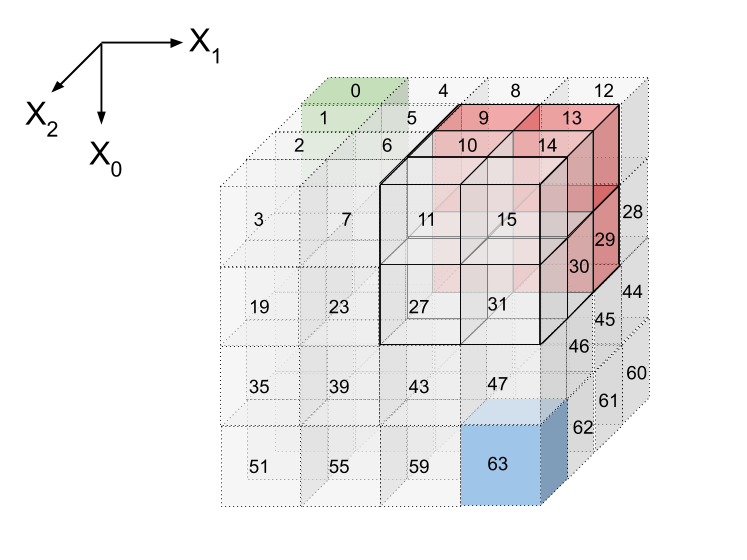
\includegraphics[scale=0.35]{./figures/figure_1.png}
  \caption{Illustration of the \texttt{C-order} in files. The left subfigure
  shows how the data is written on disk, with each cube representing a voxel.
  The green block is the first block in the C-order while the red one represents the last block.
  The right subfigure shows how reading or writing only one part of a cuboid written
  in the \texttt{C-order} can produce seeks. Each red voxel is a voxel producing a seek.}
  \label{fig:seeks_and_rowmajor}
\end{figure*}

For the sake of clarity and without loss of generality, we assume that
 files are written in row-major order (Fig.~\ref{fig:seeks_and_rowmajor},
 a.k.a ``C" order), where the fastest moving dimension in the file is the
 last dimension of the array, and the slowest moving dimension in the file
 is the first dimension of the array. This convention is for instance the
 one used in the HDF5 format ~\cite{hdf5}.

Accessing data from an array stored on disk generates seeks in two
situations: (1) when an array block is opened for reading or writing, and
(2) when the reading or writing process moves to a different address within
the block.

\subsection{The re-partitioning problem}
\begin{table}
  \caption{Notations}
  \begin{tabular}{ll}
    \multicolumn{2}{c}{\cellcolor{black!25}Mono-space fonts are used for array partitions}\\
    \texttt{A} & 3D array to repartition \\
    \texttt{inBlocks} & set of input blocks \\
    \texttt{outBlocks} & set of output blocks \\
    \texttt{readBlocks} & set of read blocks \\
    \texttt{writeBlocks} & set of write blocks \\

    &\\
    \multicolumn{2}{c}{\cellcolor{black!25}Square capitals are used for block shapes}\\
    A = ($A_0$, $A_1$, $A_2$) & shape of \texttt{A}\\
    I = ($I_0$, $I_1$, $I_2$)& shape of input blocks\\
    O = ($O_0$, $O_1$, $O_2$) & shape of output blocks\\
    R = ($R_0$, $R_1$, $R_2$) & shape of read blocks\\
    W = ($W_0$, $W_1$, $W_2$) & shape of write blocks\\
    &\\
    \multicolumn{2}{c}{\cellcolor{black!25}Round capitals are used for block end coordinates}\\

    $\mathcal{I}$ = ($\mathcal{I}_0$, $\mathcal{I}_1$, $\mathcal{I}_2$), \enskip $\mathcal{I}_d \subset \mathbb{N} $ & input block end coordinates \\
    $\mathcal{O}$ = ($\mathcal{O}_0$, $\mathcal{O}_1$, $\mathcal{O}_2$), \enskip $\mathcal{O}_d \subset \mathbb{N} $ & output block end coordinates\\
    $\mathcal{R}$ = ($\mathcal{R}_0$, $\mathcal{R}_1$, $\mathcal{R}_2$), \enskip $\mathcal{R}_d \subset \mathbb{N} $ & read block end coordinates\\
    $\mathcal{W}$ = ($\mathcal{W}_0$, $\mathcal{W}_1$, $\mathcal{W}_2$), \enskip $\mathcal{W}_d \subset \mathbb{N} $ & write block end coordinates\\
    &
  \end{tabular}
  \label{table:notations}
\end{table}
\begin{algorithm}
  \caption{General re-partitioning algorithm}
  \label{algo:generalrepartition}
  \begin{algorithmic}[1]
    \STATE \textbf{Inputs}
    \STATE inBlocks: input blocks of shape $I$, stored on disk
    \STATE outBlocks: output blocks of shape $O$, to be written
    \STATE $m$: memory available
    \STATE
    \STATE \textbf{Outputs}
    \STATE none (outBlocks are written)
    \STATE
    \STATE \textbf{Algorithm}
    \STATE readBlocks, writeBlocks $\leftarrow$ getReadWriteBlocks($I$, $O$, $m$)
    \STATE initialize(cache)
    \FOR{readBlock in readBlocks}
      \STATE data $\leftarrow$ read(readBlock, inBlocks)
      \STATE cache.insert(data)
      \FOR{writeBlock in writeBlocks}
        \IF{$\mathrm{readBlock} \cap \mathrm{writeBlock} \neq \emptyset$ \\
             \quad \textbf{and} cache.isComplete(writeBlock)}
          \STATE data $\leftarrow$ cache.pop(writeBlock)
          \STATE write(data, outBlocks)
        \ENDIF
      \ENDFOR
    \ENDFOR

  \end{algorithmic}
\end{algorithm}

\tristan{Timothée, add a figure to show input blocks, read blocks, write blocks, output blocks. Add labels to 
show that for baseline R=I et W=R, alors que pour keep, R=$\hat R$ et W=O (?)}
We focus on 3D arrays for simplicity. Consider a 3D array \texttt{A} of shape $A =
(A_i, A_j, A_k)$, partitioned as uniformly-shaped input blocks of shape $I =
(I_i, I_j, I_k)$ stored on disk. Our goal is to re-partition the input
blocks into uniform output blocks of shape $O = (O_i, O_j, O_k)$,
where $O \neq I$. Our notations are summarized in
Table~\ref{table:notations}.

We formalize the re-partitioning problem as follows.
A re-partioning algorithm (Algorithm~\ref{algo:generalrepartition}) takes a
list of input blocks \texttt{inBlocks} of shape $I$, a list of output
blocks \texttt{outBlocks} of shape $O$, and the amount of memory \texttt{m}
available for the algorithm. Subject to $m$, the algorithm determines (1)
\texttt{readBlocks}, a list of uniformly-shaped blocks of shape $R$ to be read from the
input blocks, and (2) \texttt{writeBlocks}, a list of blocks,
usually not uniformly-shaped, where each block contains a contiuous piece of
data that will be written in an output block with a single seek (line 10).
If read blocks and input blocks have a different shape, then reading read blocks requires
more than one seek. Similarly, if write blocks and output blocks have a different shape,
then writing write blocks requires more than one seek. Input, output, read
and write blocks all form a partition of the 3D array of shape $A$. The
main loop of the algorithm (line 12) loads one read block at a time (line
13), inserts it into a cache (line 14), and writes write blocks from the
cache when they are complete (lines 15 -- 20).

It should be noted that blocks are passed to the algorithm by reference,
not by data. Only variables \texttt{data} (lines 13, 17) and \texttt{cache}
(line 14) hold actual data, contributing to the consumed memory.

Since read and write blocks both represent a partition of $A$, all the
elements in \texttt{inBlocks} are read exactly once, and written exactly once too. Other
problem formalizations may allow for input elements to be read and
discarded, to reduce seeks. Exploring such a trade-off
between seeks and redundant reads could be an interesting extension to this problem.

Our goal is to minimize the number of seeks done by the algorithm, which
occur during reads (line 13) and writes (line 18). The re-partitioning
problem is therefore to find \texttt{readBlocks} and \texttt{writeBlocks} that
minimize \textsc{seeks}, the objective function that returns the number of
seeks done by the algorithm, subject to the memory constraint $m$.

% Problem: re-partitioning of multi-dimensional arrays
% Find: readBlocks and writeBlocks
% Subject to: m
% Such that: seeks is minimal
% \tristan{formalize problem definition}.

Solutions of this problem materialize as implementations of function
\texttt{getReadWriteBlocks} (Alg.~\ref{algo:generalrepartition}, line 10). A
lower bound on the number of seeks for the repartitioning problem is $n_I +
n_I$, with $n_I$ the number of input blocks and $n_O$ the number of output
blocks. Indeed, input and output files all have to be accessed at least
once, which requires a seek.

For simplicity, we require that all blocks in \texttt{readBlocks} have the
same shape $R$. We also identify the size of an array in memory as its
number of elements. To the best of our knowledge, no algorithm has been
proposed for the repartitioning problem.


\subsection{Baseline}

Our baseline algorithm for the repartitioning problem loads one input block
at a time ($R$=$I$), and directly writes it to the appropriate output
blocks ($W$=$R$). It assumes that input blocks fit in memory. The number of
generatd seeks $s_b$
depends on how write blocks overlap with
output blocks in each dimension (Fig.\ref{fig:cuts} \tristan{Timothee, faire une figure
qui represente les deux plans (X0, X1) et (X1, X2) en utilisant les notations ci-dessous}). To compute $s_b$, we define
$\mathcal{W}_d$ and $\mathcal{O}_d$ the sets of write and output block end
coordinates in dimension $d$:
\[
  \forall d \in \llbracket 1, 3 \rrbracket,
\]
\begin{equation}
  \mathcal{W}_d = \Big\{ iW_d, i \in \llbracket 1, A_d/W_d \rrbracket \Big\} \quad \mathrm{and} \quad
  \mathcal{O}_d = \Big\{ iO_d, i \in \llbracket 1, A_d/O_d \rrbracket \Big\} ~\label{eq:baseline-blocks}
\end{equation}
We then define the \emph{cuts} of the $i^{th}$ output block along dimension
$d$ as follows:
\[
  \forall i \in \llbracket 1, A_d/O_d \rrbracket,
\]
\[
  C_{i, d} = C_{i, d}\left(  \mathcal{W}_d, \mathcal{O}_d \right) = \Big\{ w \in \mathcal{W}_d, (i-1)O_d < w < iO_d \Big\}
\]
The number of output block pieces along dimension $d$ is then:
\[
  c_d = c_d\left(  \mathcal{W}_d, \mathcal{O}_d \right) =
               \sum_{i=1}^{A_d/O_d} \vert C_{i, d}\left(  \mathcal{W}_d, \mathcal{O}_d \right) \vert + 1 - \delta_{\vert C_{i, d}\left(  \mathcal{W}_d, \mathcal{O}_d \right) \vert, 0}
\]
where $\vert$ . $\vert$ is the cardinality operator and $\delta$ is the Kronecker delta.
The number of matching endings is:
\[
  m_d = m_d\left(  \mathcal{W}_d, \mathcal{O}_d \right) = \vert \mathcal{W}_d \cup  \mathcal{O}_d \vert  - c_d
  \]
Finally, the number of seeks created by the baseline algorithm is:
\begin{equation}
  s_b = A_0 A_1 c_2 +
      A_0 c_1 m_2 +
      c_0 m_1 m_2
       + n_i + n_o \label{eq:seeks-baseline}
\end{equation}


As can be seen from Equation~\ref{eq:seeks-baseline}, cuts along dimension 2 generate $\mathcal{O}(A_0 A_1)$
seeks, which is prohibitive when \texttt{A} is large, cuts along dimension 1 generate $\mathcal{O}(A_0)$ seeks and cuts in
dimension 0 generate $\mathcal{O}(1)$ seeks. The \keep heuristic described
in the next section aims at avoiding cuts primarily in dimension 2, and if
possible in dimension 1 and 0. An experimental verification of the model will be provided in
Section ~\ref{sec:experiments}.




% We implemented Equation~\ref{eq:1} and ran it on a cubic array to confirm these
% theories. One shape mismatch is added at a time in order to see the impact on
% the number of seeks. The setting and results of this simulation are summarized
% in table~\ref{tab:simseekmodel}.

% \begin{table}[ht]
%   \centering
%   \caption{Results of the simulation using the baseline algorithm's seek model}

%    \begin{tabular}[t]{| c | c | c | c | c |}
%    \hline
%    Mismatch & R & B=I & O & nb seeks \\
%      \hline\hline
%      k & (3500,3500,3500) & (500,500,875) & (500,500,500) & 73,500,000 \\
%      \hline
%      j & (3500,3500,3500) & (500,875,500) & (500,500,500) & 147,000 \\
%      \hline
%      i & (3500,3500,3500) & (875,500,500) & (500,500,500) & 294 \\
%      \hline
%      i,j & (3500,3500,3500) & (875,875,500) & (500,500,500) & 147,168 \\
%      \hline
%      i,j,k & (3500,3500,3500) & (875,875,875) & (500,500,500) & 73,584,096 \\
%      \hline
%    \end{tabular}

%    \label{tab:simseekmodel}

% \end{table}

%----------------------------------------
\section{The \keep heuristic}
%----------------------------------------
\tristan{Timothée, remplacer $\Lambda$ par $\hat R$ dans toutes les figures (notation plus claire)}
As mentioned previously, the baseline strategy empties
the cache at each iteration, which generates many seeks when input and output 
blocks have different shapes. Instead, the proposed
\keep heuristic keeps in cache the array elements that cannot be written
contiguously to the output blocks.

\subsection{Overview}

\begin{algorithm}
  \caption{\keep heuristic (implements \texttt{getReadWriteBlocks}) \tristan{verify all line numbers in the text, they have changed}}
  \label{algo:keep}
  \begin{algorithmic}[1]
    \STATE \textbf{Inputs}
    \STATE inBlocks: input blocks of shape $I$, stored on disk
    \STATE outBlocks: output blocks of shape $O$, to be written
    \STATE $m$: memory available
    \STATE
    \STATE \textbf{Outputs}
    \STATE readBlocks: a list of read blocks
    \STATE writeBlocks: a list of write blocks
    \STATE
    \STATE \textbf{Algorithm}
    \STATE readShapes = candidateReadShapes($I$, $O$)
    \STATE minSeeks = None
    \FOR{$R$ in readShapes}
      \STATE readBlocks = blocks($R$, $A$)
      \STATE writeBlocks = createWriteBlocks(readBlocks, outBlocks)  \tristan{OR JUST OUTBLOCKS???}
      \STATE mc = peakMemory($R$)
      \IF{mc > m}
      \STATE \textbf{continue} \COMMENT{Read shape cannot respect memory constraint}
      \ENDIF
      \IF{$R$ == $\hat R$}
      \STATE bestReadBlocks = readBlocks
      \STATE \textbf{break} \COMMENT{$\hat R$ respects memory constraint}
      \ENDIF
      \STATE s = generatedSeeks($I$, $R$, writeBlocks, $O$)
      \IF{minSeeks == None or s' < minSeeks}
      \STATE minSeeks, bestReadBlocks = s, readBlocks
      \ENDIF
    \ENDFOR
    \RETURN readBlocks, writeBlocks
  \end{algorithmic}
\end{algorithm}
The \keep heuristic (Alg.~\ref{algo:keep}) is a brute-force search of the
best read shape among a list of candidates (line 11). For each candidate
read shape, it creates an ordered list of read blocks (line 14), defines
write blocks accordingly (line 15), evaluates the peak memory consumed by
this solution (line 16), and provided that the memory constraint is
respected, computes the number of seeks (line 24), and selects the read
shape that minimizes the number of seeks (line 25-27).

The \keep heuristic uses the following functions, described in the
remainder of this section: \texttt{candidateReadShapes} (line 11), \texttt{blocks} (line 14),
\texttt{createWriteBlocks} (line 15), \texttt{peakMemory} (line 16),
\texttt{generatedSeeks} (line 24).

\subsection{Candidate read shapes}

% Read shape candidates are generated as to avoid cuts along dimension 2
% during reads and writes. Ideally, the read shape would cover an exact
% number of input blocks, to avoid seeks during reads, and would include at
% least one output block, to avoid seeks during writes. In practice, this
% might not be possible due to memory limitations, since at each iteration
% the parts of the read block that are not written must remain in cache.

To generate candidate read shapes, we first define a shape $\hat R$ such
that in each dimension $d$, $\hat R_d$ is the smallest multiple of $I_d$
that is greater or equal to $O_d$:

\[
\forall d \in \{1, 2, 3\},
\]
\[
  \enskip \exists \hat k \in \mathbb{N}, \enskip \hat R_d = \hat kI_d \enskip \mathrm{and} \enskip \hat k I_d \geq O_d \enskip \mathrm{and} \enskip \forall k < \hat k, \enskip kI_d < O_d
\]

Using $\hat R$ as read shape minimizes the seeks in the input blocks, as
in this situation each iteration reads input blocks completely, requiring a
single seek per input block. If there is enough memory to use write blocks
of shape $O$, then this solution also minimizes the seeks in the output
blocks, as output blocks can be written in a single seek too \tristan{isn't it always the case?}.

Function \texttt{getCandidateReadShape} returns the following shapes:
\[
  \Big\{ (C_0, C_1, \hat R_2) \in \mathbb{N}^3 \enskip / \enskip
          \forall i \in \{1, 2\}, \enskip \exists k_i \in \mathbb{N}, \enskip
           A_i = k_iC_i \enskip \mathrm{and} \enskip C_i \leq \hat R_i \Big\}
\]
The third coordinate of all read shapes is set to $\hat R_2$, to guarantee
that no cuts along dimension 2 will be made during reads. This assumes that
$m > \hat R_2$, i.e., a block of shape (1, 1, $\hat R_k$) fits in
memory, which is reasonable. The other two coordinates are set to divisors of $A_0$ and $A_1$ which are
less than or equal to $\hat R_0$ and $\hat R_1$ (respectively).

The candidate shapes are sorted first by decreasing $C_1$ values, then by
decreasing $C_0$ values. The first tested read shape is therefore
$\hat R$. While $\hat R$ is the optimal read shape, leading to a single
seek per input or output block, there is no obvious relation between the
other candidate shapes and the number of seeks that they generate, since
this number depends on how input, read, write, and output block shapes are
arranged. For this reason, the \keep heuristic returns if $\hat R$
respects the memory constraint (line 20), but it otherwise evaluates all
the other read shapes.

\subsection{Block order}

While creating uniform block coordinates from a block shape is
straightforward, their order may have an impact on the amount of data
stored in cache and therefore on the peak memory consumption. For
simplicity, function \texttt{block} returns read blocks in the
order used for array elements on disk (C order in this paper). 

\subsection{Creation of write blocks}

Function \texttt{createWriteBlocks} returns write blocks created from read and output blocks
as follows. For each read block,
eight write blocks are first created, defined as the $F_i$ blocks in
Figure~\ref{fig:nomenclature_overlaps}. The $F_i$ blocks are then merged
recursively with sub-blocks of neighboring read blocks, following the rules
in Table~\ref{tab:fusion}. The resulting write blocks cover complete output blocks. \tristan{if this is the case we should just 
say that from the beginning and move the Fi definition back to the memory consumption and remove this section because there's nothing to say.}
\tristan{du coup, si on garde toutes les chutes en mémoire et qu'on les fusionne comme ça, 
je ne comprends pas comment on peut avoir des seeks en sortie car on va recréer exactement les output blocks.}
\begin{table}
  \centering
  \caption{Recursive merging of initial write blocks. The first column
  identifies a sub-block of a read block (i.e., an initial write block),
  and the second column identifies the sub-block(s) of the neighboring read
  block(s) that are merged with the sub-block of the first column. For instance, sub-block $F_1$ is merged with sub-block $F_0$ 
  of the neighboring read block in dimension $X_2$.}
   \begin{tabular}{c|l}
   \rowcolor{black!25}
   Sub-block & Merged with \\
   \rowcolor{black!25}
             & (sub-block, neighbor direction) \\
   $F_0$     & -- \\
   \rowcolor{black!10}
   $F_1$     & ($F_0$, $X_2$) \\
   $F_2$     & ($F_0$, $X_1$) \\
   \rowcolor{black!10}
   $F_3$     & ($F_1$, $X_1$), ($F_2$, $X_2$) \\
   $F_4$     & ($F_0$, $X_0$) \\
   \rowcolor{black!10}
   $F_5$     & ($F_1$, $X_0$), ($F_4$, $X_2$)\\
   $F_6$     & ($F_2$, $X_0$), ($F_4$, $X_1$)\\
   \rowcolor{black!10}
   $F_7$     & ($F_3$, $X_0$), ($F_5$, $X_1$), ($F_2$, $X_2$)\\
   \end{tabular}
   \label{tab:fusion}
\end{table}

\begin{figure*}[h]
  \centering
  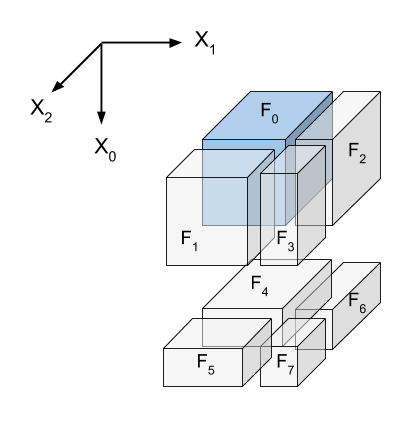
\includegraphics[scale=0.4]{./figures/figure_3.png}
  \caption{Illustration of an input aggregate (left) and its division into indexed remainder volumes (right).
  Each remainder volume is a part of an output block. \tristan{Timothée,
  update figure as discussed}\tristan{Comment peux-tu supposer que les
  origines du read block et de l'output block sont superposées et qu'il n'y
  a donc pas de chute "avant" F0 ?}}
  \label{fig:nomenclature_overlaps}
  \end{figure*}

\subsection{Peak memory}

To determine the peak memory used by a particular combination of read and
write blocks, one needs to determine the amount of data in the cache at
each iteration, which depends on how read and write blocks overlap. Since we were only able to find an analytical
upper bound of the peak memory usage, which in fact largely overestimates
it, we instead simulate each iteration of the \keep heuristic to measure
the cache size.

The simulation requires $\vert \texttt{readBlocks} \vert$ iterations. It
assumes that (1) read blocks are in the order used for array elements on
disk (C order in this paper), consistently with function \texttt{blocks}
and (2) write blocks are defined as described in the previous section
\tristan{or just out blocks?}. Under these assumptions, we note that the
maximum number of sub-blocks of each type stored in the cache at any given
iteration is 1 for sub-blocks of type $F_1$, $A_2/R_2$ for sub-blocks of
type $F_2$ or $F_3$, and $A_1/R_1A_2/R_2$ for sub-blocks of type $F_4$ to
$F_7$. The simulation is therefore implemented with 3 circular buffers
$B_1$, $B_2$, $B_3$ of size 1, $A_2/R_2$ and $A_1/R_1A_2/R_2$ respectively.
At each iteration, the size of $F_1$ is added to $B_1$, the size of $F_2
\cup F_3$ is added to $B_2$, and the size of $F_4 \cup \ldots \cup F_7$ is
added to $B_3$. The sum of elements in $B_1$, $B_2$ and $B_3$ is computed
and its max across all iterations is returned as the peak memory
consumption.

\subsection{Number of generated seeks}

Similar to the
baseline, seeks generated by the \keep heuristic happen during reads (line
13 in Alg.~\ref{algo:generalrepartition}) and during writes (line 18). The
seeks generated during writes are directly obtained from
Equation~\ref{eq:seeks-baseline}, defining $\mathcal{W}_d$ as the end coordinates of
\texttt{writeBlocks}. To count the seeks generated
during reads, we note that the read process is dual to the write process:
writing in-memory blocks with end coordinates $\mathcal{M}$ to disk blocks
with end coordinates $\mathcal{D}$ generates the same number of seeks as
reading disk blocks with end coordinates $\mathcal{D}$ to in-memory blocks
with end coordinates $\mathcal{M}$. This number of seeks is returned by the following function:

\begin{eqnarray*}
  \textsc{seeks} \left(  \mathcal{M}, \mathcal{D} \right) &=&  A_0 A_1 c_2\left(\mathcal{M}_d, \mathcal{D}_d\right) + \\
                                                         &&  A_0 c_1\left(\mathcal{M}_d, \mathcal{D}_d\right) m_2\left(\mathcal{M}_d, \mathcal{D}_d\right) +\\
                                                         && c_0\left(\mathcal{M}_d, \mathcal{D}_d\right) m_1\left(\mathcal{M}_d, \mathcal{D}_d\right) m_2\left(\mathcal{M}_d, \mathcal{D}_d \right)\\
                                                         && + \vert \mathcal{D} \vert
\end{eqnarray*}
Equation~\ref{eq:seeks-baseline} becomes:
\[
  s_b = \textsc{seeks} \left( \mathcal{W}, \mathcal{O} \right) + n_i
\]
where $\mathcal{W}$ and $\mathcal{O}$ are defined as in
Equation~\ref{eq:baseline-blocks}. It should be noted that function
\textsc{seeks} does not assume that $\mathcal{M}$ or $\mathcal{O}$ relate to
blocks of uniform shape. Therefore, it can be applied to the \keep
heuristics where write blocks are not necessarily of uniform shape.
The number of seeks generated by the \keep algorithm is given by:
\begin{equation}
  s_k = \textsc{seeks} \left(  \mathcal{R}, \mathcal{I} \right) + \textsc{seeks} \left( \mathcal{W}, \mathcal{O} \right) \label{eq:seeks-keep}
\end{equation}
where the first term represents the number of seeks required to read input
 blocks of end coordinates $\mathcal{I}$ into read blocks of end
 coordinates $\mathcal{R}$, and the second term represents the number of
 seeks required to write write blocks of end coordinates $\mathcal{W}$ into
 output blocks of end coordinates $\mathcal{O}$. Function
 \texttt{generatedSeeks} is
 a direct implementation of Equation~\ref{eq:seeks-keep}.

\subsection{Implementation}

\tristan{Timothée, I would feel better if you could use the implementation
of function seek in seek\_tristan.py in your implementation. It should be giving the same results as yours,
but probably faster.}

We implemented the baseline and \keep heuristic in Python 3.7. The
\href{https://github.com/GTimothee/repartition_experiments}{project's
repository} \tristan{Move to big-data-lab-team} includes documentation on
how to install the package and its dependencies. The code used in the
experiments is also available in the same repository \tristan{is it still
the case?}.

The implementation supports the HDF5 file format, but the code is modular
enough to support other formats in the future.

% \subsection{Optimizing the bruteforce search}
\tristan{Tristan to reword this paragraph when the comments are clarified}
One can note that when the read buffer shape $B$ is smaller than $\hat R$,
the overall number of buffers increases.
It is therefore quicker to compute the number of seeks and the maximum
quantity of memory to be used for the buffers close to $\hat R$.
On the contrary, it can take several seconds to compute theses metrics \tristan{seeks should be really fast with the model} for
small buffers, knowing that among the possible buffer shapes, it is not rare to
see buffers like ($1,1,\hat R_k$), which is the worst case.
That is why we decided, instead of testing all possible buffer shapes, to start
testing the shapes from the ideal ones ($\hat R$) to the worst ones
($1,1,\hat R_k$ for example), reducing the buffer shape in the $j$ dimension
first, and then in $i$.
We only estimate the amount of seeks to be produced if the maximum quantity
to be consumed is smaller than $m$ \tristan{redundant with algorithm 2}.
We also added a heuristic in order not to test all shapes when it is more
probable that the best shapes are closer to $\hat R$.
In this spirit, we added a maximum number of iteration above which the search
is stopped if no improvement in the number of seeks has been found.
We set this limit to 10 buffers \tristan{This heuristic should either be removed (preferred)
or explained in details}.

%----------------------------------------
\section{Experiments}
%----------------------------------------
\label{sec:experiments}
\subsection{Seek model validation}

\tristan{generate 1,000 random shapes, compute number of seeks with models for baseline and keep,
check that implementation makes the same number}

\subsection{Experiment conditions}
The experiments were run on a node of a private cluster with 256~GB of RAM,
6 SSDs of size 480~GB and 32~cores \tristan{report SSD and CPU models,
Linux distribution, kernel version, file system}. We only used 1 node and 1
SSD at a time \tristan{is it true for the large image?}. The cluster was
accessed through the SLURM batch manager.

We repartitioned an array of shape $A=(3500,3500,3500)$ and of type
\texttt{float16} (2 bytes per array element \tristan{the block sizes in Table 3 correspond to
1 byte per array element, please check.}), representing \todo{X}~GB,
using the input and output block shapes in Table~\ref{tab:exp}.
\tristan{Was compression used?} \tristan{Describe the other, larger array.}


We measured repartitioning time for $m$=256~GB, 8~GB and 4~GB. The memory
was controlled through SLURM's cgroup-based memory requirement, which means
that $m$ was the total amount of RAM allocated to the repartitioning task,
including anonymous memory and cache. Swapping was disabled.

The buffer shapes of each run for each amount of RAM available are summarized in
Table~\ref{tab:buffer_shapes} \tristan{I don't get what this buffer shape is.
is it the best read shape found by the keep algo? If so, these are results, not experiment conditions.}.

\begin{table}[ht]
  \centering
  \caption{Input and output block shapes for $A=(3500,3500,3500)$.}
   \begin{tabular}{c|cc|cc}
   \rowcolor{black!25}
          & \multicolumn{2}{c|}{\texttt{inBlocks}} & \multicolumn{2}{c}{\texttt{outBlocks}} \\
    \rowcolor{black!25}
     \#     & $I$ & size (MB) & $O$ & size (MB)  \\
   \hline
   0 & (875,875,875) & 670 & (875,1750,875) & 1340 \\
   1 &               &     & (700,875,700)  & 429 \\
   \rowcolor{black!10}
   2 & (350,350,350) & 43  & (500,500,500)  & 125 \\
   \rowcolor{black!10}
   3 &               &     & (250,250,250)  & 16  \\
   4 & (175,175,175) &  5  & (250,250,250)  & 16 \\
   \rowcolor{black!10}
   5 & (350,875,350) & 107 & (500,875,500)  & 219 \\
   \rowcolor{black!10}
   6 &               &     & (350,500,350)  & 61 \\
   \end{tabular}
   \label{tab:exp}
\end{table}


\begin{table}[ht]
  \centering
  \caption{Description of the different buffer shapes used for each run by the keep algorithm, depending on the amount of RAM available. The last column gives the maximum RAM consumption estimated by the keep algorithm before running (at buffer selection time).}

   \begin{tabular}[t]{| c | c | c | c |}
   \hline
   $m$ & ref & buffer shape & maximum estimated (MB) \\
   \hline
   \multirow{2}{*}{256GB} & 0 & (875, 1750, 875) & 2,679.6875 \\
   & 1 & (875, 875, 875) &  14,631.09375 \\
   & 2 & (700, 700, 700) &  11,596.0 \\
   & 3 & (350, 350, 350) &  5,255.75 \\
   & 4 & (350, 350, 350) &  5,255.75 \\
   & 5 & (700, 875, 700) &  10,920.0 \\
   & 6 & (350, 875, 350) &  1,133.125 \\
   \hline
   \multirow{2}{*}{8GB} & 0 & (875, 1750, 875) & 2,679.6875 \\
   & 1 & (700, 875, 875) &  1,715.0 \\
   & 2 & (500, 700, 700) &  2,040.0 \\
   & 3 & (350, 350, 350) &  5,255.75 \\
   & 4 & (350, 350, 350) &  5,255.75 \\
   & 5 & (500, 875, 700) &  962.5 \\
   & 6 & (350, 875, 350) &  1,133.125 \\
   \hline
   \multirow{2}{*}{4GB} & 0 & (875, 1750, 875) & 2,679.6875 \\
   & 1 & (700, 875, 875) &  1,715.0 \\
   & 2 & (500, 700, 700) &  2,040.0 \\
   & 3 & (250, 350, 350) &  430.0 \\
   & 4 & (250, 350, 350) &  430.0 \\
   & 5 & (500, 875, 700) &  962.5 \\
   & 6 & (350, 875, 350) &  1,133.125 \\
   \hline
   \end{tabular}

   \label{tab:buffer_shapes}

\end{table}

\subsection{Results}
\tristan{Figures should be made nicer. Suggestion: make it similar to panels (a) and (b) in figure 2 of https://www.nature.com/articles/nmeth.3041}

\tristan{Reword to start with the main result, then describe the details}

% commenter sur l'accélération générale (moyenne)
% focus sur les writes
%  pas de seek pour le write.
% évolution en fonction de la qté mémoire, mention page cache
% variability between the runs

The results in terms of processing times are shown on
Figure~\ref{fig:results}, whereas the results in terms of seeks are
presented on Figure~\ref{fig:seeks_results}.

Looking at Figure~\ref{fig:results}, we can see that
the baseline algorithm performs surprisingly well compared to the keep algorithm
when the main memory available is 256GB (all the node's available RAM).
We can see that when the amount of RAM available decreases (8 and 4GB), the
performances of the baseline algorithm decreases drastically.
In particular, the keep algorithm is approximately 2 times faster for runs
2, 3 and 4 on Figure~\ref{fig:results4}.
From these observations we suppose that the baseline algorithm performs well
with 256GB because it leverages the page cache.
It is counter-intuitive to see that the performances of the baseline algorithm
differs for the different amount of RAM available, because apart from $m$
nothing changes for the baseline algorithm; the read buffer shape stays $B=I$.

Another factor for the baseline algorithm to perform well compared to the
keep algorithm with 256GB is the time overhead of the keep algorithm which is
very important as one can see on Figure~\ref{fig:results}.
This is due to our implementation and the tradeoff presented in section
``Implementation".
Concretely, the time overhead is mainly due to making copies of the data from
the read buffers to the cache.
In terms of read/write processing time however, we can clearly see an
important speedup by the keep algorithm compared to the baseline for
runs 3 and 4 (Figure~\ref{fig:results}).
One can also notice a non-negligible speedup for runs 1 to 5 for the experiment
with 8 (Figure~\ref{fig:results8}) and 4GB (Figure~\ref{fig:results4}).
There are big differences in the benefits of using the keep algorithm instead of
the baseline algorithm, depending on the different runs.
This is due to the difference in complexity between the runs.
The runs that are more complex (with more shape mismatches) are more optimized
by the keep algorithm, hence producing a bigger speedup from the keep compared to
the baseline.

Considering Figure~\ref{fig:seeks_results}, one can see that the number of
seeks is drastically reduced by the keep algorithm, which is consistent with
the results in terms of processing time.
We remark that one needs to reduce significantly the amount of seeks produced
by a re-partition algorithm to clearly see an impact on the processing time.
Considering run 4 which shows the most important differences in terms of
processing time, the amount of seeks have been reduced from about 100 millions
seeks to thousands of seeks.
We also remark that although the number of seeks have been reduced from millions
to thousands of seeks for runs 1 to 5, the reduction in processing time does not
follow linearly the reduction in the number of seeks.
This is probably due to the fact that some seeks are more costly than others,
which has not been taken into account in our problem formulation.

\begin{figure*}
     \centering
     \begin{subfigure}[b]{\textwidth}
         \centering
         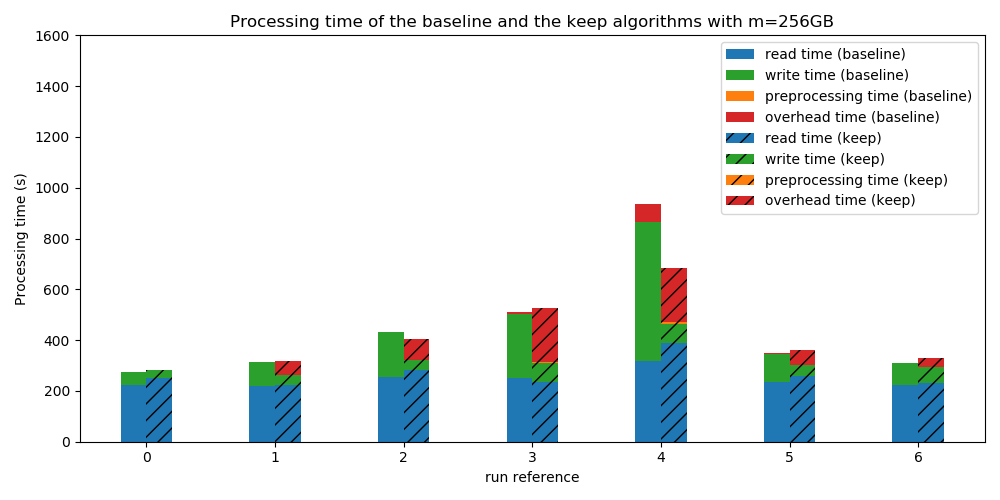
\includegraphics[scale=0.5]{./figures/results_256.png}
         \caption{Processing times for $m=256$GB}
         \label{fig:results256}
     \end{subfigure}
     \vfill
     \begin{subfigure}[b]{\textwidth}
         \centering
         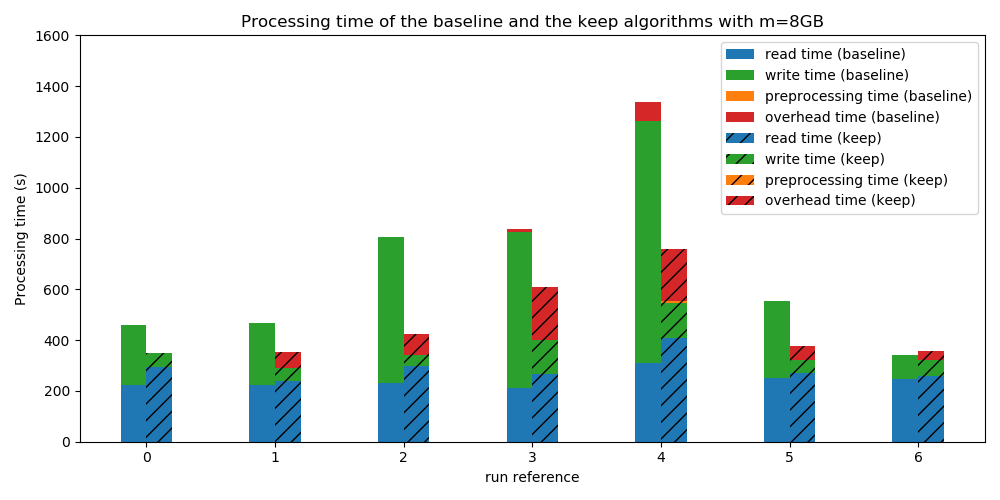
\includegraphics[scale=0.5]{./figures/results_8.png}
         \caption{Processing times for $m=8$GB}
         \label{fig:results8}
     \end{subfigure}
     \vfill
     \begin{subfigure}[b]{\textwidth}
         \centering
         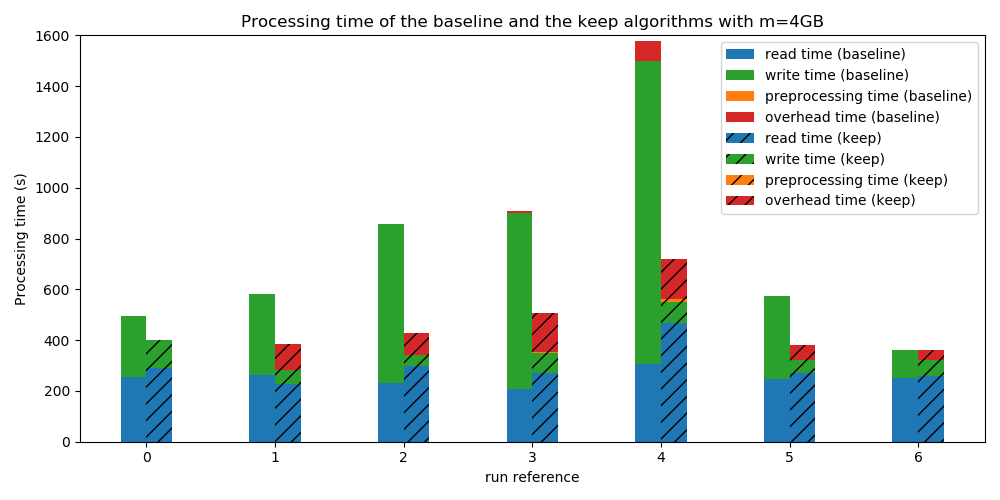
\includegraphics[scale=0.5]{./figures/results_4.png}
         \caption{Processing times for $m=4$GB}
         \label{fig:results4}
     \end{subfigure}

     \caption{Results in terms of processing time for the keep and baseline algorithms. From top to bottom, the results are presented for 256, 8 and 4GB of available main memory.}
     \label{fig:results}

\end{figure*}

\begin{figure*}
     \centering
     \begin{subfigure}[b]{\textwidth}
         \centering
         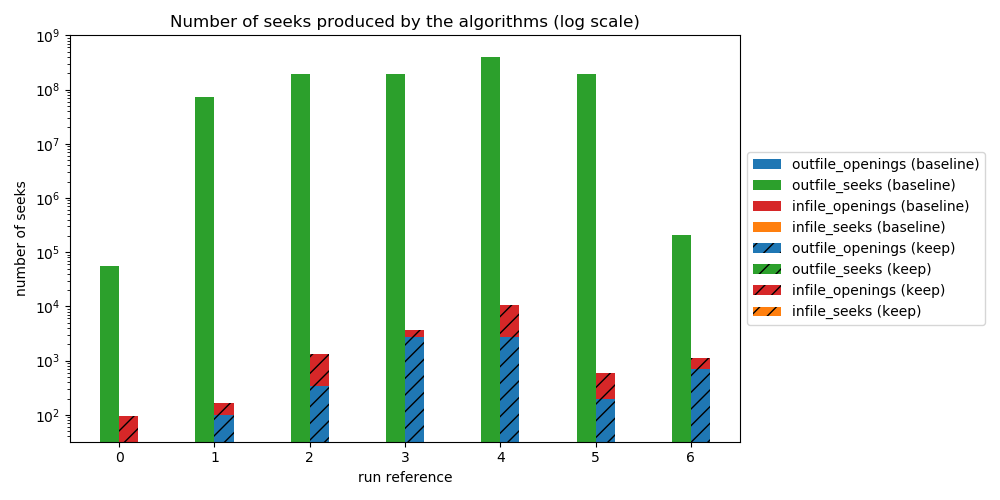
\includegraphics[scale=0.5]{./figures/results_seeks_256.png}
         \caption{Seek quantities for $m=256$GB}
         \label{fig:seeks256}
     \end{subfigure}
     \vfill
     \begin{subfigure}[b]{\textwidth}
         \centering
         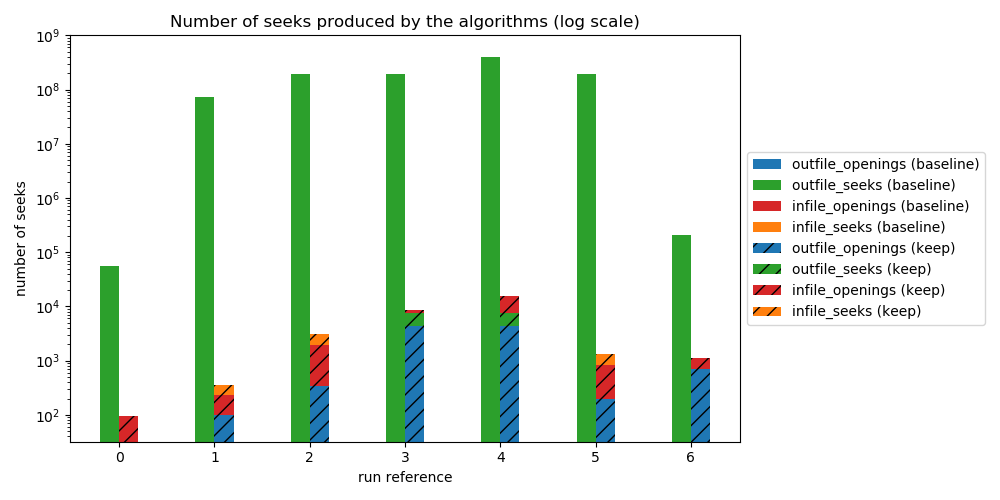
\includegraphics[scale=0.5]{./figures/results_seeks_8.png}
         \caption{Seek quantities for $m=8$GB}
         \label{fig:seeks8}
     \end{subfigure}
     \vfill
     \begin{subfigure}[b]{\textwidth}
         \centering
         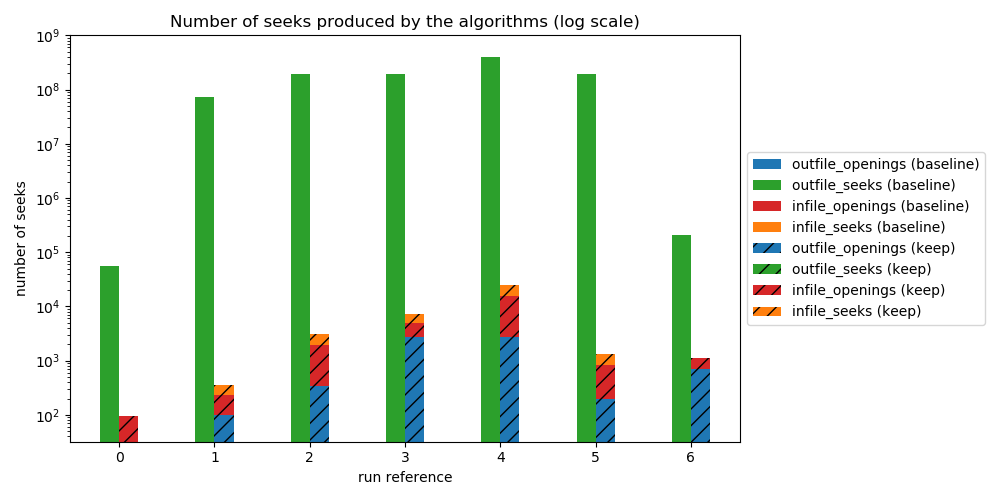
\includegraphics[scale=0.5]{./figures/results_seeks_4.png}
         \caption{Seek quantities for $m=4$GB}
         \label{fig:seeks4}
     \end{subfigure}

     \caption{Results in terms of seeks for the keep and baseline algorithms. From top to bottom, the results are presented for 256, 8 and 4GB of available main memory.}
     \label{fig:seeks_results}
\end{figure*}

%----------------------------------------
\section{Discussion}
%----------------------------------------
\tristan{Tristan to refocus the discussion and conclusion}
\tristan{From discussion with Valerie, mention practical considerations related to page cache and readahead}

\subsection{On the keep algorithm}
The keep algorithm can reduce the number of seeks produced by a re-partition
problem from millions to thousands of seeks, compared to the baseline algorithm.
Even if the write time has been drastically reduced on the results shown on
Figure~\ref{fig:results}, there is still margin for improvement in optimizing
the read time.
Finally, it could be interesting to try identifying the type of seeks that are
more costly than the others and focus future implementations of the re-partition
algorithm to reduce such costly seeks.

Although the keep algorithm can be 2 times faster than the baseline algorithm
in some cases, our implementation suffers from a tradeoff between optimizing
the processing time and predicting the maximum amount of memory consumed.
In some non-complex cases, the baseline algorithm can be as efficient as the
keep algorithm.
Moreover, the baseline algorithm seems to take advantage of the surplus of
main memory available in the node, although in theory it is supposed to use
only the size of one input block in bytes at a time.
This does not seem to be the case of the keep algorithm for which the maximum
amount of main memory consumed can be estimated before run.

\subsection{The buffer ordering problem}
The buffer order is important when using the keep strategy, as it defines when
a piece of data will be loaded and when a write buffer will be complete, hence
ready to be written down and freed from the cache.
Representing the read buffers by a complete bidirectional graph in which each
vertex is a buffer, we can model the problem as kind of a complex shortest path
problem.
Indeed, for a given buffer shape $B$, we want to find the read buffers order
that will keep the amount of memory used by the re-partition algorithm low.
Solving this problem would incur more infering at runtime and a potentially
complex algorithm to run.
We decided to keep things simple using a naive buffer order, as the goal of
this study was primarily to assess if the keep algorithm works.

\subsection{The split and merge problems}

Special cases of the re-partitioning problem occur when $I=A$ (``split'' problem)
or when $O=A$ (``merge'' problem). Two strategies were introduced
in~\cite{seqalgorithms} to address these problems: the ``multiple" and the
``clustered" strategies. In these strategies, every read block is directly written to the
destination output files, that is, \texttt{readBlocks} and \texttt{writeBlocks} are identical ($R=W$).
The only difference between the multiple and the clustered strategies lies in
the selection of $R$.

In the split problem, the naive
strategy defines the read blocks as having the same shape as the output blocks
($R$=$O$). The read blocks are iteratively loaded from $A$ and entirely written
to the appropriate output block.
The clustered strategy, however, loads as
many contiguous read blocks of shape $O$ as possible to fit in $m$.
$R$ is therefore a multiple of $O$.
Depending on the amount of main memory available, read blocks may be loaded
individually, by entire block columns, or by entire block slabs.
Although this strategy allows to write each output block in one seek, the clustered strategy is limited by the fact
that it does not optimize the reading step.
In the general re-partitioning problem, one can expect the clustered strategy to
perform poorly as
(1) it reads an output block regardless of its spread among input blocks
and (2) even if it is stored in one input block the algorithm will do a lot of seeks in
case of a shape mismatch \tristan{I dont get (2), to be clarified}.

The multiple strategy
aims at not doing any seek while reading \textit{and} writing:
both the input and the output blocks are read/written contiguously. In
terms of Algorithm~\ref{algo:generalrepartition}, it means defining read blocks as
contiguous parts of the input array and write blocks as contiguous parts of
the output arrays. It is equivalent to extending the buffer \tristan{read blocks or write blocks?} in the inverse of
the storage order: $k \rightarrow j \rightarrow i$ in the case
of the \texttt{C-order}. Although the multiple strategy does not seek while reading or writing, it
requires many switches between output blocks, which also requires seeking.

\subsection{Impact of the buffer order on performance}
Using the keep strategy, one may order the buffer loadings to reduce the maximum
quantity of extra data stored in memory, hence, reducing the amount of seeks.
For example, if the shape mismatches occur only in the $k$ axis, loading the
buffers in this direction will enable recycling the extra data in cache,
resulting in a smallest memory consumption over time.
The memory saved thanks to a smart
ordering could enable the storage of more extra data in memory using the
keep strategy, further reducing the amount of seeks produced.

As explained in the discussion, the buffer ordering problem is complex and does
not seem easily solvable.
This study uses a naive order which is, again, the inverse storage order.
The reason for that order is that as it is more important to keep data in the
$k$ dimension to save seeks and we assume that $B_k=\hat R_k$, it seems
reasonable to load the buffers in the $k$ dimension first.
Note that using such
an order recycles extra data in the $k$ dimension first; It is therefore
more efficient when the biggest shape mismatch between the input and output
blocks is in $k$.

Thanksfully, the impact of the buffer ordering on performance can be
mitigated. Indeed, the impact of the buffer ordering depends on the size of the
mismatches. One can reduce the amount of extra data by using smallest blocks: Even
if the overlap between the input and output files is big with respect to their
size, the area/volume of the overlap will be kept small.

\subsection{ROI extraction problem}
The Region Of Interest (ROI) extraction problem is a related problem that still
needs to be adressed.
A solution using chunking as been introduced in~\cite{optimal_chuking}.
The authors define an array partitioned into chunks of equal shapes and then
define a query as an arbitrary subarray of the input, chunked, array.
They define the optimal chunking problem as finding the optimal chunk such
that the expected number of chunks retrieved to answer the query is minimal.

In our opinion, the solution in~\cite{optimal_chuking} is limited due to the
need of historical or theoretical workload and the necessity to repartition the
input array into an ``optimal" chunk shape.
We would prefer letting the application choose the appropriate chunk shape
regarding its needs and not needing to estimate the processing workload.
We define the ROI extraction problem as follows: Finding an algorithm that takes
as input an arbitrary chunk shape and extract the ROI data from the chunks with
the less number of seeks as possible.

\subsection{Solving three problems at once}
As stated in the introduction, the split and merge tasks are special cases of
the repartition task. This observation leads us to think that maybe one could find
one optimal algorithm for the split, merge and repartition tasks.

If we were to use the keep algorithm with $I=R$, we would read the input data
in slices, exactly like the multiple strategy. The only difference between the
two strategies, however, is that if some remainders appear at the bottom of the
buffer, the keep algorithm would keep it to try to read and write files in one
seek. Not only the keep algorithm tries to limit seeking into the files but it
also tries to limit switching between the files. It would be interesting to
compare the two algorithms for the split/merge tasks to see if the keep
implementation brings similar results or any kind of improvement.

\subsection{The dask Python package}
\texttt{dask} is a popular Python package, part of the SciPy ecosystem, enabling
parallel and out-of-core computations~\cite{matthew_rocklin-proc-scipy-2015}.
It has an important scientific community which is likely to have the problem we
try to solve in this paper, i.e. re-partitioning multidimensional array files.
That is why we would find it interesting to implement our work as an optimization
package for \texttt{dask}.
In particular, we would focus on the \texttt{dask.array} collection, a data
structure designed for multi-dimensional array processing using blocked
algorithms.

\texttt{dask} represents computations as task graphs that are dynamically executed by one
of several schedulers including the single-threaded, the multi-threaded, the
multi-process, and the distributed schedulers. Custom schedulers can also be
implemented. \texttt{dask} graphs can be used out-of-the-box or through
built-in APIs. A \texttt{dask} graph is implemented in plain Python as a
dictionary with any hashable as keys and any object as values. More precisely,
a ``Value" is any object different than a task and a ``Task" is a tuple with a
callable as first element. Examples of APIs/collections include
\texttt{dask.array}, a parallel and out-of-core
Numpy clone, and \texttt{dask.dataframe}, a Pandas clone.
Our first prototype of implementation of the keep algorithm is showing promising
results in optimizing the computation graphs produced by \texttt{dask}.

\subsection{Towards distributed systems}
As most of the big data processing is now done on clusters, it could be interesting
to find distributed versions of the split/merge/re-partition algorithms.
Lots of scientists use HPC (High Performance Computing) clusters regularly which
brings considerations about how to use such distributed algorithms with Lustre
for example, a commonly used filesystem for HPC.

\texttt{dask} also provides a distributed scheduler that seems to be quite
efficient.
It is now recommended for use, even on local computers (using one node).

\subsection{Limit to our implementation}
We encountered a tradeoff in the implementation of the keep algorithm which
makes its processing time longer that it could be.
Indeed, we had to implement the keep algorithm by passing data per value from
the read buffers to the cache, instead of by address.
This is due to our formulation of the re-partition problem which requires us to
be able to predict the amount of memory consumed by our algorithm to ensure that
the limit $m$ will be respected.
Python uses a custom garbage collector which manages the release of our
data structures and prevents us to force the release of some data parts.
We found that copying the data to the cache enabled us to stay below the
maximum memory consumption that we predicted at the buffer selection time.


%----------------------------------------
\section{Conclusion}
%----------------------------------------

Multidimensional array chunking is a routine for scientists nowadays.
That is why efficiently processing such arrays is of major importance in the big data era.

Splitting and merging arrays has been successfully done, we therefore attempted
to solve the next step: the re-partitioning problem.
This problem consists in efficiently re-writing a chunked array to change the blocks shape.
We think that solving this problem could enable us to solve the ROI (region of interest)
extraction problem in the future, which is also a very common problem for scientists.
We formally defined the re-partitioning problem together with a \emph{baseline algorithm} to solve it.
We also presented the \emph{keep algorithm} to reduce the number of seeks produced during
the re-partitioning and hopefully reduce the processing time of such task.
The keep algorithm reduces the number of seeks by
(1) constraining the read buffers shape to minimize the read time, and
(2) leveraging a ``cache" to minimize the write time.

Although the re-partitioning problem is more complex than splitting/merging chunks,
we proved that it can be optimized and that it is possible to reduce the
processing time significantly.
Surprisingly however, the baseline algorithm has been found to perform pretty
well when there is a lot of memory available as it leverages the page cache to
speedup computations without reducing the number of seeks.
For now, the keep algorithm may be more interesting than the baseline algorithm
only when the memory constraint is important ($m$ small compared to the array size).

In the future, the algorithm performances may be improved by finding a variant
to the keep algorithm that also reduce the read time significantly,
identifying and focusing on reducing the most expensive seeks,
and finally, finding parrallel and/or distributive versions of the keep algorithm.

%----------------------------------------
\section{Acknowledgments}
%----------------------------------------

The computing platform was obtained with funding from the Canada Foundation for Innovation.

\tristan{Timothée, make sure that all references have a title, date, and venue (journal or conference name).
Check capitalization of words like HDF5, etc}

\bibliography{Bibliography}
\bibliographystyle{ieeetr}

\end{document}
